\section{Results}\label{Sec_Results}

As already indicated, the selected behaviors that we modeled are the choices of three movie genres: drama, action and comedy. In this section we list and briefly explain the results of the TPB models fitting the user data (acquired by the designed questionnaire).  For each of the six models that we fitted and tested (three models from attributes, one from norms and control, and the top level aggregate model) we fitted the MVR model (resulting in the model coefficients $\beta_k$ and the proportion of the explained variances $R^2$) and we performed the linear discriminant analysis (resulting in the discriminant weights $w_k$ and the separability $s$ in terms of the Fisher discriminant analysis \cite{RencherChristensen201207}). We do not report the results for all six models, but only for the cognitive attributes (selected for demonstrating how to interpret the results) and for the aggregate model which summarizes the whole TPB model. 


\subsection{Selected sub-model: the cognitive dimension of attitudes}\label{SubSec_CogAttr}

This sub-model explains the role and contribution of the user's answers to eight questions $Q_1 - Q_8$ regarding the cognitive dimension of attitudes (i.e. the selection of a movie of one of the selected genres). In Fig. \ref{Fig_AggregModel}, which depicts the aggregated model, this sub-model is located on the top of the three sub-models explaining the user's cognitive dimension of attributes.

The proportion of the explained variance for the cognitive dimension of attitudes is $R^2=0.48$. This high value allows us to interpret the beta coefficients of the model and determine the relative importance of the cognitive attitude in the overall mode as discussed in Subsec. \ref{SubSec_AggregateModel}.

The normalized MVR model coefficients are listed at Tab. \ref{Tab_attitudeCog_MvRegress}. The coefficient $\b_0$ 
represents the offset of the resulting model, while the coefficients $\b_k$, $1\leq k \leq 8$ correspond to the questions $Q_k$. The significant $\b$ coefficients at risk level $\a=0.05$ are marked with $^*$. 
\begin{table}[!h]
  \centering
   \begin{tabular}{|l|c|c|c|c|c|c|c|c|c|}
\hline
\textbf{Genre} &\textbf{$\beta_{0}$}&\textbf{$\beta_{1}$}&\textbf{$\beta_{2}$}&\textbf{$\beta_{3}$}&\textbf{$\beta_{4}$}&\textbf{$\beta_{5}$}&\textbf{$\beta_{6}$}&\textbf{$\beta_{7}$}&\textbf{$\beta_{8}$}\\\hline\hline
\textbf{Drama}&0.32&0.02&-0.03&-0.01&-0.02&0.01&0.00&-0.01&0.00\\\hline
\textbf{Action}&3.43&0.09&-0.11$^*$&0.10$^*$&0.05&-0.08&0.13$^*$&-0.02&-0.02\\\hline
\textbf{Comedy}&3.69&0.48$^*$&-0.34$^*$&0.05&0.07&-0.04&-0.12$^*$&-0.11$^*$&0.06\\\hline
\end{tabular}

  \caption{MVR coefficients of the cognitive dimension of the attitudes predictors, $R^2 = 0.48$.}
  \label{Tab_attitudeCog_MvRegress}
\end{table}
We observe that none of the coefficient that model the genre Drama is significant and therefore no conclusion can be made here. This is most probably due to the relatively low sample size used to fit the model. Regarding the genre Action, the coefficients representing $Q_2=${\it How important for you is the story in the movie?}, $Q_3=${\it How important for you is the movie's genre?} and $Q_6=${\it How important for you are the special effects?} are significant. Since $\b_2$ is negative, the users that do not care much about the story of the movie are more likely to select the drama genre. The positive coefficients $\b_3$ and $\b_6$ show that the users that cared about the genre and the special effects are more likely to select the drama genre. 

In the same way we interpret the selection of Comedy movies. The large positive coefficient $\b_1=0.48$ representing $Q_1=${\it How important for you is the main actor of the movie?} indicates that the main actor is the most important factor in selecting the comedy genre, while the coefficient $\b_2$ representing $Q_1=${\it How important for you is the story in the movie?} indicates that the story has very little relevance in selecting the comedy genre. the coefficients $\b_6=-0.12$ and $\b_7$ representing the questions $Q_6=${\it How important for you are the special effects?} and $Q_7=${\it How important is an attractive trailer?}, respectively, indicate the low relevance of the special effects and of the trailer in the selection of the comedy genre. 

We analyzed the separability of the genre selection behaviors by LDA. The Fisher separability of the cognitive dimension of attitudes is $s = 0.81$ which means a moderate separability. The LDA coefficients separating the given pairs of genres are listed in Tab. \ref{Tab_attitudeCog_LDA}. The significant coefficients at the risk level $\a=0.05$ are labeled by $^*$. A significant contribution to the separation of the genres Drama and Action are obtained from $Q_3$ and $Q_6$ etc. 

\begin{table}[!h]
  \centering
   \begin{tabular}{|l|c|c|c|c|c|c|c|c|}
\hline
\textbf{Genre pair}&\textbf{$w_{1}$}&\textbf{$w_{2}$}&\textbf{$w_{3}$}&\textbf{$w_{4}$}&\textbf{$w_{5}$}&\textbf{$w_{6}$}&\textbf{$w_{7}$}&\textbf{$w_{8}$}\\\hline\hline
\textbf{Drama/Action}&-0.87&-0.82&-3.26$^*$&-0.66&-0.42&-3.54$^*$&1.68&-0.01\\\hline
\textbf{Drama/Comedy}&-5.67$^*$&-0.49&0.94&0.09&-1.48&-1.23&1.19&-1.56\\\hline
\textbf{Action/Comedy}&-4.80$^*$&0.32&4.19$^*$&0.75&-1.07&2.31&-0.49&-1.55\\\hline
\end{tabular}

  \caption{Linear discriminant coefficients of the cognitive dimension of attitudes predictors.}
  \label{Tab_attitudeCog_LDA}
\end{table}

To summarize the interpretation, the questions and underlying decision factors that are relevant in both models (MVR and LDA) are regarded as the most important. These are the $Q_1$, $Q_3$ and $Q_6$ factors. The question $Q_1$ is the most important one since it is involved in the discriminant function with highest magnitudes. The behavior of selecting the Drama genre is not predicted well (no significant MVR coefficient) while the behavior of selecting the comedy genre is predicted well. 

\subsection{Aggregated TPB model}\label{SubSec_AggregateModel}

We computed the scores predicted by each of the beliefs, norm and control models and used them as predictors for the three behaviors to build a hierarchical model. Each of the underlying models contributed three scores, one for each of the behaviors. The obtained aggregated model achieves a large proportion of explained variance $R^2=0.89$ and a good Fisher separability value of $1.008$. The aggregated model with $R^2$ of the sub-models are depicted in Fig. \ref{Fig_AggregModel}. 

 \begin{figure}[h!]
 \begin{center}
   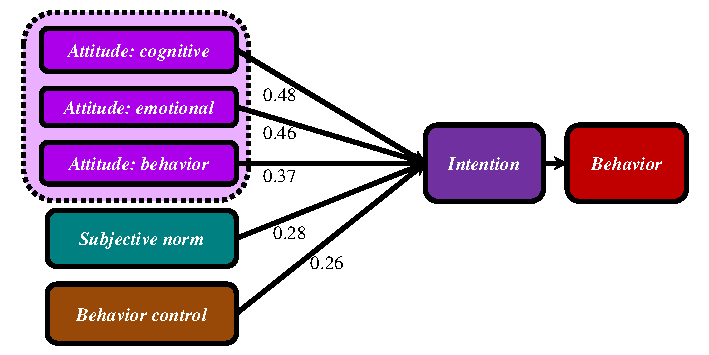
\includegraphics[width=9cm]{TpbTopH.pdf}
   \caption[Fig_AggregModel]{Aggregated  model of genre selection, $R^2=0.89$.}
   \label{Fig_AggregModel}
 \end{center}
 \end{figure}


We do not list and interpret the coefficients of MVR and LDA for the aggregated model here. We summarize the whole model by a list of the explained variances and Fisher separabilities in Tab. \ref{Tab_all_R2andSeps}. All the listed $R^2$ values including the aggregated $R^2=0.89$ are statistically significant and they indicate the relative weight of each sub-model in the movie selection of the genre. Behavior control contributed the least and the cognitive aspect of attributes contributed the most to the whole model. Note that for the sake of simplicity we did not regress behavior intentions but directly the behaviors themselves. The models allows to regress the intentions but this it is beyond the scope of this paper. 

\begin{table}[!h]
  \centering
   \begin{tabular}{|l|c|c|c|c|c|}
\hline
&\textbf{Attr: cog.}&\textbf{Attr: emot.}&\textbf{Attr: behav.}&\textbf{Norms}&\textbf{Cont.}\\\hline\hline
$\textbf{R}^2$&0.49&0.46&0.37&0.28&0.26\\\hline
\textbf{Separability}&0.81&1.03&0.60&0.44&0.50\\\hline
\end{tabular}

  \caption{Proportion of the Explained variance $R^2$ and Fisher separability for the aggregated model.}
  \label{Tab_all_R2andSeps}
\end{table}

% - hierarchy
% - model selection

 

